\documentclass[12 pt]{article}
\usepackage[utf8]{inputenc}
\usepackage{filecontents}
\usepackage[many]{tcolorbox}
\usepackage{graphicx}
\usepackage{harpoon}
%\usepackage{apacite} 
\usepackage{xcolor}
\usepackage{latexsym}
\usepackage{amssymb}
\usepackage{amsmath}
\usepackage{mdframed}
%\usepackage[authoryear]{natbib}
\usepackage{hyperref, url}
\usepackage[show]{ed}
\usepackage{subfigure}
\usepackage[ntheorem]{empheq} 
\usepackage{amsthm, amssymb, amsfonts, latexsym}
\usepackage{pst-all}

\usepackage{enumitem}

\setlength{\parskip}{1.7em}
\setlength{\parindent}{0em}


%\setlength{\baselineskip}{20pt}

\setlength{\textwidth}{429.75499pt}
\setlength{\textheight}{643.20255pt}
\setlength{\oddsidemargin}{5 mm}
\setlength{\evensidemargin}{5 mm}
\setlength{\topmargin}{0 mm}
\setlength{\headsep}{0 mm}
\setlength{\headheight}{0 mm}



\newcommand{\citealtt}[1]{\citeauthor{#1},\citeyear{#1}}
\newcommand{\myycite}[1]{\citep{#1}}

\mathchardef\mhyphen="2D

%\newcommand{\cev}[1]{\reflectbox{\ensuremath{\vec{\reflectbox{\ensuremath{#1}}}}}}


\usepackage{pst-node,graphicx,pst-blur}
%\uspackage{auto-pst-pdf}
%\usepackage{tikz-cd} 



\makeatletter
\DeclareRobustCommand{\cev}[1]{%
  \mathpalette\do@cev{#1}%
}
\newcommand{\do@cev}[2]{%
  \fix@cev{#1}{+}%
  \reflectbox{$\m@th#1\vec{\reflectbox{$\fix@cev{#1}{-}\m@th#1#2\fix@cev{#1}{+}$}}$}%
  \fix@cev{#1}{-}%
}
\newcommand{\fix@cev}[2]{%
  \ifx#1\displaystyle
    \mkern#20mu
  \else
    \ifx#1\textstyle
      \mkern#20mu
    \else
      \ifx#1\scriptstyle
        \mkern#26mu
      \else
        \mkern#26mu
      \fi
    \fi
  \fi
}

\makeatother

\newcommand{\xcm}{\epsfxsize=3.1cm}
\newcommand{\fig}[1]{\epsfbox}
% \newcommand{\bp}{\begin{minipage}{3.1cm}}
% \newcommand{\ep}{\end{minipage}}



\newtheorem{Definition}{Definition}[]
%\newmdtheoremenv{Theorem}{Theorem}[]
\newtheorem{Theorem}{Theorem}[]
\newtheorem{Lemma}{Lemma}[]
\newtheorem{Proposition}{Proposition}[]
\newtheorem{Corollary}{Corollary}[]
\newtheorem{Remark}{Remark}[]
\newtheorem{Example}{Example}[]


%Shortcut symbols
\newcommand{\Ftheta}{\ensuremath{F_\theta}}


\makeatletter 
\renewcommand{\thefigure}{\@arabic\c@figure}
\makeatother
\usepackage{xr}


%%%% PNAS GRAPHICS SETUP- FROM THE PNAS STYLE LATEX FILE
\RequirePackage{graphicx,xcolor}
\RequirePackage{colortbl}
\RequirePackage{booktabs}
\RequirePackage{algorithm}
\RequirePackage[noend]{algpseudocode}
\RequirePackage{changepage}
\RequirePackage[twoside,%
				letterpaper,includeheadfoot,%
				layoutsize={8.125in,10.875in},%
                layouthoffset=0.1875in,%
                layoutvoffset=0.0625in,%
                left=38.5pt,%
                right=43pt,%
                top=43pt,% 10pt provided by headsep
                bottom=32pt,%
                headheight=0pt,% No Header
                headsep=10pt,%
                footskip=25pt,
                marginparwidth=38pt]{geometry}
\RequirePackage[labelfont={bf,sf},%
                labelsep=period,%
                figurename=Fig. ]{caption}
\setlength{\columnsep}{13.5pt} % Distance between the two columns of text
\setlength{\parindent}{12pt} % Paragraph indent

%% Figure caption style
\DeclareCaptionFormat{pnasformat}{\normalfont\sffamily\fontsize{7}{9}\selectfont#1#2#3}
\captionsetup*{format=pnasformat}

%%% GREYBOX AROUND FIG
\definecolor{lightgray}{gray}{0.95}
\newcommand\greybox[1]{%
  \vskip\baselineskip%
  \par\noindent\colorbox{lightgray}{%
    \begin{minipage}{\textwidth}#1\end{minipage}%
  }%
  \vskip\baselineskip%
}

\newtcolorbox{paperbox}[1][]{
    enhanced,
    colback=white,
    boxrule=0pt,
    boxsep=0pt,
    arc=0mm,
    width=0.8\linewidth,
    fuzzy shadow={0mm}{-4pt}{-4pt}{1mm}{black!30!white},
    #1
}


\externaldocument{Supp_Koopman-0808}
\begin{document}



\title{Project Thesis/Report}



\author{} 
\date{}
\date{}
\maketitle

\section{Introduction}

Experimenting on biological, physical, and artificial systems in order to generate a more informative dynamical model is a well-established practice in modern science. Traditional methods for modelling physical systems are based on laws of physics that are based either on empirical relationships or on intuition. For systems that evolve with time, physical laws yield mathematical equations that govern how the quantities evolve with time. However our world around is, for the most part, much more complex than that which can be distilled into elegant equations. We do not fully understand many of the more complex systems, nor do they even provide us with a good physical intuition of the underlying principles governing the dynamics.

To complicate this - the underlying systems we observe often display sensitive dependence on initial conditions; despite having highly similar initial conditions, differing orbits diverge quickly and to such an extent that it becomes seemingly impossible to retrace their steps back to the original conditions. Even the presence of usually 'negligible' computational noise or measurement error renders long-term point-wise prediction infeasible. 
There are many difficulties that one encounters while modelling such systems:
\vspace{-8mm}
\begin{enumerate}[noitemsep, label=\roman*.]
  \item One may not have access to the complete states of the systems
  \item The actual system may be described by functions that behave wildly in the sense their graphs have a wild oscillatory behaviour, i.e., they have a large functional complexity.    
\end{enumerate}


Models derived primarily from data can be classified into three categories: 
\vspace{-8mm}
\begin{enumerate}[noitemsep, label=\roman*.]
  \item  Interpretable models (i.e., they establish relationships between internal physical mechanisms), 
  \item Partially interpretable models capturing some modes of the dynamics, 
  \item Non-Interpretable models, defined as such mainly due to the fact that they are defined on a different phase space that is usually high-dimensional. 
\end{enumerate}

Examples in the literature attempting to forecast data from such systems have tried a number of different approaches with differing degrees of success. One could learn a system conjugate to the underlying system by applying the Takens delay embedding; this learnt system could then be used for forecasting the original system. \cite{takens1981detecting}. An ordinary differential equation can be obtained from data (Citations to Sindy). Alternatively, one could approximate the vector field by a library of functions (Citations to Sindy) to obtain interpretable models. Takens delay methods suffer from lack of robustness to noise and may not yield a learnable map that has lower functional complexity (See Section 3). For the methods that build interpretable models (Citations to Sindy) the complete system states are needed which is rarely available. Pure machine learning methodology that processes temporal information (like the echo state networks (Citations to echo state networks)) is an approach that maps data onto a higher dimensional space for further processing. Although they perform  well on forecasting some dynamical systems, they fail completely on others (Citations here) as there is often guarantee that the right function was learnt during training.

Recent partially interpretable models available in the literature have been based on the Koopman operator (e.g.,\cite{koopman1932dynamical,budivsic2012applied}) to  employ observables mapping the data onto a higher-dimensional space. This then makes the dynamics in the higher-dimensional space more amenable for approximation by a linear transformation. Such methods, obviously, do not guarantee an exact reconstructions for nonlinear models, and in practice provide poor long-term consistency for a large class of systems. (Add citation)

The non-interpretable models include the delay embedding and the machine learning algorithms. Under some generic conditions, the Takens delay embedding theorem \cite{takens1981detecting} and its various generalisations (e.g., \cite{sauer1991embedology, stark1999delay, gutman2018embedding, gutman2018embedding}) establishes the learnability of a system constructed by concatenating sufficiently large previous time-series observations of a dynamical system into a vector (called delay coordinates). This then establishes the existence of a map on the space of delay coordinates equivalent (or topologically conjugate) to the underlying map from which the observed time-series was first obtained. Although topological conjugacy guarantees an alternate representation of the underlying system, the quality of thsi representationstill depends on numerous parameters, making the comprehension of the dynamics rather unreliable (e.g., \cite{principe1992prediction}). One reason for this fragility is that the embedded attractor in the reconstruction space not always an attractor itself, despite  unquestionably being an invariant set. Since the embedded object is not \textbf{(definitely/always?)} an attractor (as explained in Chapter 3) it can cause predictions to fail.


Practically, the application of Takens embedding involves learning a map through some technique and consequently one wishes that these would have low functional complexity\cite{manjunath2021universal}, i.e., functions with fewer oscillatory graphs.

This thesis deals with the implementation and analysis of non-interpretable models that can guarantee \textbf{exact/accurate} reconstruction. The project work concerns the study and implementation of a method (Citation to paper with Adriaan) that incorporates learning a function by mapping the data on to a higher dimensional space. With a clear understanding of how the data is mapped onto the higher dimensional space, the method then permits the learning of a dynamical system topologically conjugate to that of the underlying system. Instead of linear regression, deep learning methods are employed to learn the correct function. With slight modifications to the implementation in the paper (with Adriaan), we show that one can construct accurate non-interpretable models with the ability to reconstruct attractors from more hard-to-forecast systems like the double pendulum. (The forecasting of the time-series from a double pendulum has not been reported before.) Moreover, we also demonstrate that long-term statistical consistency is preserved.

By solidifying the mathematical underpinnings of our theory, we hope to guarantee the ability to construct models with predictive power ranging from molecular biology to neuroscience. in the near future. (We can modify this sentence when the report is completed.)

The report is organised as follows: 
\newline In Section 2, we recall the definition of a discrete-time dynamical system, how a discrete-system arises from a flow of an ODE and then proceed to define the inverse limit space and topological conjugacy of autonomous systems. 
\newline In Section 3, we introduce the problem of forecasting dynamical systems, state the Takens delay embedding theorem and discuss various issues faced while forecasting. 
\newline In Section 4, a driven dynamical system is defined and discuss the properties of a specific class of driven dynamical systems that we make use of in this thesis/report/paper. 
\newline Finally in Section 5 we show the implementation of these forecasting methods, and conclusions are provided in Section 6.


\section{Discrete-time Dynamical Systems}

In this chapter, we provide a brief description of what a discrete-time dynamical system is and what it means for it to exhibit chaos. We refer to \cite{devaney2018introduction, de2013elements} for more details. 

At its most elementary level, a dynamical system is just something that evolves deterministically through time. In the context of this thesis, deterministic refers to the fact that a system evolves according to specified rules rather than based on random events. 
Dynamical systems arise in a variety of situations. A continuous dynamical system, and here specifically the motion of a pendulum, is one in which quantities such as the angular position and angular momentum are known at all times. 
The equations of the dynamical system take the form of one or more ordinary differential equation that determine the relevant quantities at any future time if we know the initial location and momentum. 
In ecology, discrete dynamical systems are widely used to model population growth. The model in this case is a function calculating the following generation's population given the population of the previous generation. If we know the starting population, we may once again calculate the population at any time in the future. 

Formally, a function $T: U \to U$, where $U$ is some set is  a \emph{discrete-time dynamical system} and its iterates $\{u,Tu,T^2u,\ldots\}$, where $T^n$ denotes the $n$-fold composition of $T$ with itself, describe the evolution of an initial condition $u\in U$ (Note that we drop the brackets and denote $T(u)$ by $Tu$ for simplicity).  





Continuous dynamical systems modelled using ordinary differential equations can give rise to discrete-time dynamical systems. To see this, consider differential equation $\dot{x} = f(x)$, $f: \mathbb{R}^n \to \mathbb{R}^n$, $n\in\mathbb{N}$ given to have a unique solution passing through 
each point $x\in\mathbb{R}^{n}$, the flow of the equation \label{defn_flow} is defined to be a mapping $\varphi: \mathbb{R}^n \times \mathbb{R} \to \mathbb{R}$ that satisfies the following properties:
\vspace{-8mm}
\begin{enumerate}[noitemsep, label=\roman*.]
  \item $x(t)$ is a solution of the differential equation,
  \item $x(0)=x_0$, and
  \item $\varphi(x_0,t) = x(t)$.
\end{enumerate}
By fixing $t=K$, we can define the \emph{time-$K$ map} as  $T(x):= \varphi(x_0,K)$, and it is easily verified that $T\circ T(x_0) = \varphi(x_0,2K)$. In general the $m^{th}$ iterate of $x_0$ under $T$ would be the value of the solution of the ODE evaluated at time $mK$ with the initial condition $x_0$. 
Thus ordinary differential equations give rise to a discrete-time dynamical systems by sampling the value of $x$ at time intervals $K$ units apart. 

Of course, discrete-time dynamical systems need not always arise through a differential equation, and once again we may consider the field of ecology where discrete dynamical systems are often directly derived or assumed. 
\emph{There is a school of thought that advocates discrete-time dynamical systems to be more natural for modelling real-world observations than differential equations (see \cite{saber2010introduction})}. \textbf{too philosphical, or actually good?}

A numerical discretization of a differential equation can also give rise to a discrete-time dynamical system. For instance, Euler's method approximates $\dot{x}(t)$ by $(x(t+h)-x(t))/h$; if $h$ is fixed throughout, the solution of a differential equation $\dot{x}=f(x)$ 
can be approximated at the time instant $t+(m+1)h$ by iterating the equation 
$$x(t+(m+1)h) = x(t+mh) + h f(x(t+mh)).$$ 
Adopting more succinct notation by replacing $x(t+mh)$ with $u_m$, we rewrite the above equation as
$$u_{m+1} = u_m + hf(u_m)$$
or, in even simpler terms, as the discrete-time dynamical system with map $T(u) = u + hf(u)$, where $T$, $u$ and $f$ are understood to be as above.

\subsection{Invariant Sets}

A core concept in the study of dynamical systems is that of invariance. Given a discrete-time dynamical system $T: U \to U$, a subset $A \subset U$ is said to be an \emph{invariant set} if $T(A) =A$. 
We also define the \emph{orbit of T} to be a sequence $\bar{u} = \{u_n\}_{n\in \mathbb{Z}}$ obeying the update equation, $u_{n+1}=Tu_n$, $n \in \mathbb{Z}$. 


Two examples of invariant sets include a fixed point where $Tu=u$ for  $u\in U$, and a periodic orbit, i.e., a set of iterates $\{u,Tu, T^2u,\ldots,T^pu\}$, where $T^{p+1}u=u$ for some $p$.  The entire space $U$ could be also be invariant.
Consider for example the space $U=[0,1]$, where $Tu=4u(1-u)$ and then $U$ is invariant. \emph{(as every $u\in{U}$ can be written as $u = 4x(1-x)$ for some $x\in{U}$)}

We may learn a great deal about the iterates of a dynamical system by considering the types of invariant sets of a discrete-time dynamical system.  For example, if $U=[0,1]$ has map $Tu= u/2$, then the only invariant set is $\{0\}$, and all orbits approach this invariant set as time flows in the forward direction. 
Indeed, if a some non-zero invariant set (call it $B$) exists, then there is  some $r\in(0,1]\cap{B}$. But $r\notin{T(B)}$ since any orbit with initial value $r$ will be a decreasing sequence. Moreover, every orbit of T will be decreasing and therefore approach the value $0$ as $n\rightarrow\infty$

One may ask if every orbit approaches an invariant set? In general the answer is no, since for the dynamical system $Tu=2u$, any orbit that does not intersect the invariant set $\{0\}$, will not approach any invariant set. 

However,  when the space $U$ is compact, all orbits approach an invariant set. \textbf{For let $\bar{u} = \{u_n\}_{n\in \mathbb{Z}}$ be an orbit in the compact space U, then $\bar{u}$ has a convergent subsequence }

In fact the $\omega$-limit set $\omega(u;T)$ of a point $u$ defined to the collection of limit points of the sequence $\{x,Tu,T^2u,\ldots\}$ is nonempty, and $\omega(u;T)$ is invariant. \textbf{(not relevant other than being an additional example perhaps?)}

We discuss various properties of invariant sets: Invariant sets can be attracting or repelling depending on how orbits in its vicinity behave (recall the examples $Tu =u/2$ and $Tu=2u$). We are interested in attractive invariant sets, and in particular so-called attractors which we define below.
\begin{Definition} \rm Let $T: U \to U$, where $U$  is a metric space with metric $d$. A compact subset $A \subset U$ is said to be an attractor if it satisfies the three conditions: 
  \vspace{-8mm}
  \begin{enumerate}
	\item $A$ is invariant. 
	\item $A$ is asymptotically stable, i.e., for every $\epsilon > 0$ and for all $u$ so that $d(u,A) < \epsilon$, we have $d(T^nu,A) \to 0$ as $n\to \infty$. 
	\item $A$ has Lyapunov stability, i.e., for every $\epsilon > 0$  there exists a $\delta(\epsilon) > 0$ so that $d(u,A) < \delta$ implies $d(T^nu,A) < \epsilon$ for all $n\ge 0$.  
\end{enumerate}
\end{Definition} 

In our previous examples, the system  $Tu=u/2$ had the singleton set $\{0\}$ as an attractor. For the system,  $Tu=4u(1-u)$ on $[0,1]$, one may easily verify that the only attractor is the entire space $[0,1]$. \textbf{For let $B$ be an attractor of U. From above, we know that B is itself invariant, is asymptotically stable and has Lyapunov stability. Now suppose there is some attractor $C\subsetneq{U}=B$, so there is a $b\in{U}$ which is not in $C$. ........  }

A dynamical system can have several attractors, and may also be contained in another attractor. 

% If the dynamics on the attractor are somewhat complicated in the sense that the attractor cannot be decomposed further, and if the attractor is infinite then there is a possibility of complicated dynamics, and a particular well-studied phenomenon of such complexity gives rise to what is called a chaotic behaviour. 

If the dynamics on an attractor cannot be decomposed further and the attractor is itself also infinite, then there is a possibility of complicated dynamics, and a particular well-studied phenomenon of such complexity gives rise to what is called chaotic behaviour. 

\subsection{Chaos}

\textbf{$\downarrow$ - should one add paragraphs like these?}
\newline In the 1960s, a number of mathematicians and mathematically interested scientists independently discovered chaos in the mathematical sense. The meteorologist Edward Lorenz may have been the first to explain this phenomenon in his 1963 paper \cite{lorenz1963deterministic}. The notions of invariance, attractivity and chaos may also bedescribed for continuous systems, and Lorenz's system comprised of a system of differential equations. The narrative of Lorenz's discovery of chaos, as well as the history of other forerunners in this subject, are fascinating. For those who are interested, we highly recommend James Gleick's book Chaos: The Making of a New Science \cite{gleick2008chaos}. It clearly illustrates these experiences, explains why chaos was such a startling and crucial mathematical and scientific discovery, and describes the underlying mathematical notions for non-specialists.

There are several intricately different notions of chaos, with each of them indicating some complexity. \textbf{ $\leftarrow  $ what are we saying here?} In practice, it is not possible to verify which notion is satisfied when data is observed from a dynamical system. We do, however, specifically recall the definition of chaos in the sense of Devaney \cite{devaney2018introduction,de2013elements} so as to understand some nuances. Devaney's definition consists of three parts, with the first being the notion  of sensitive dependence on initial conditions. 

\begin{Definition} \rm 
A dynamical system $T: U \to U$ is said to have sensitive dependence on initial conditions (SDIC) if there exists a $\delta > 0$ such that for every $u \in U$ and in every neighborhood of $u \in U$ there exists a $v\in{U}$ and an integer $N:=N{(u,v)}\in\mathbb{Z}$ such that $d(T^Nu,T^Nv)>\delta$. 	
\end{Definition}

It is important to acquire a sense of this definition as it can easily be misunderstood. It is common misconception to interpret SDIC as two close points ($u$ and $v$) that eventually become separated by a distance $\delta$ under iteration by $T$. But this is not true. To fully comprehend all the subtleties of the concept, one needs to discuss it more thoroughly by considering each sentence with care and attention, whereafter one may examine how they fit together to convey the concept of sensitive dependence. 
\textbf{ $\leftarrow$ is this talking too simply perhaps?}. 

To this end we make 3 remarks:
\vspace{-5mm}
\begin{enumerate}
  \item First, the $\delta>0$ in the definition of SDIC is independent of $u$. 
  \item Second, in every neighborhood of $u$, we may not necessarily find all points $v$ in the neighborhood distinct from $u$ that would separate from the forward iterates of $u$. 
  \item  Finally, $N$ depends upon $u$ and $v$ chosen, and their iterates may not separate for ever (i.e., for all $n>N$) and we allow their iterates to get arbitrarily close in the future. 
\end{enumerate}


 
\ednote{M: It is probably best to see a few numerical simulations to understand SDIC. (Please use the logistic map and perhaps the trajectories of the double pendulum data). } 

The second part in Devaney's definition of chaos concerns topological transitivity.

\begin{Definition}
	A dynamical system $F: U \to U$ is topologically transitive if for any pair of nonempty open sets $E_1$ and $E_2$ there exists a $n\in\mathbb{N}$ such that $T^n(E_1) \cap E_2 \not= \emptyset$. 
\end{Definition}

Topologically transitivity implies that the iterates of an open set of initial conditions gets mixed up with other open sets. On a compact metric space, it can be shown that topological transitivity also implies the existence of a point whose forward iterates are dense; or in other words, the orbit going through this point will be dense in the compact metric space. 

In fact, it is topologically more likely that the choice of an arbitrary point will be one  whose iterates are almost dense.
% I inserted a definition here: it makes more sense to me. 
\begin{Definition}
A compact metric space $U$ is said to be almost dense if the complement of the set of points which are dense in $U$ may be written as a countable union of sets of with empty interior. In other words, the set on points not dense on $U$ is topologically insignificant.
\end{Definition}

We may now define the notion of Chaos as formulated by Devaney\cite{devaney2018introduction}.
\begin{Definition}
	A dynamical system $T: U \to U$ is said to exhibit chaos in the sense of Devaney if it satisfies the three properties:
	\vspace{-5mm}
  \begin{enumerate}
		\item $T$ has SDIC.
		\item $T$ is topologically transitive.
		\item The set of periodic points of $T$ are dense in $U$. 
	\end{enumerate}
\end{Definition}


\begin{figure}[ht]
  \centering
  \begin{minipage}{.5\textwidth}
    \centering
    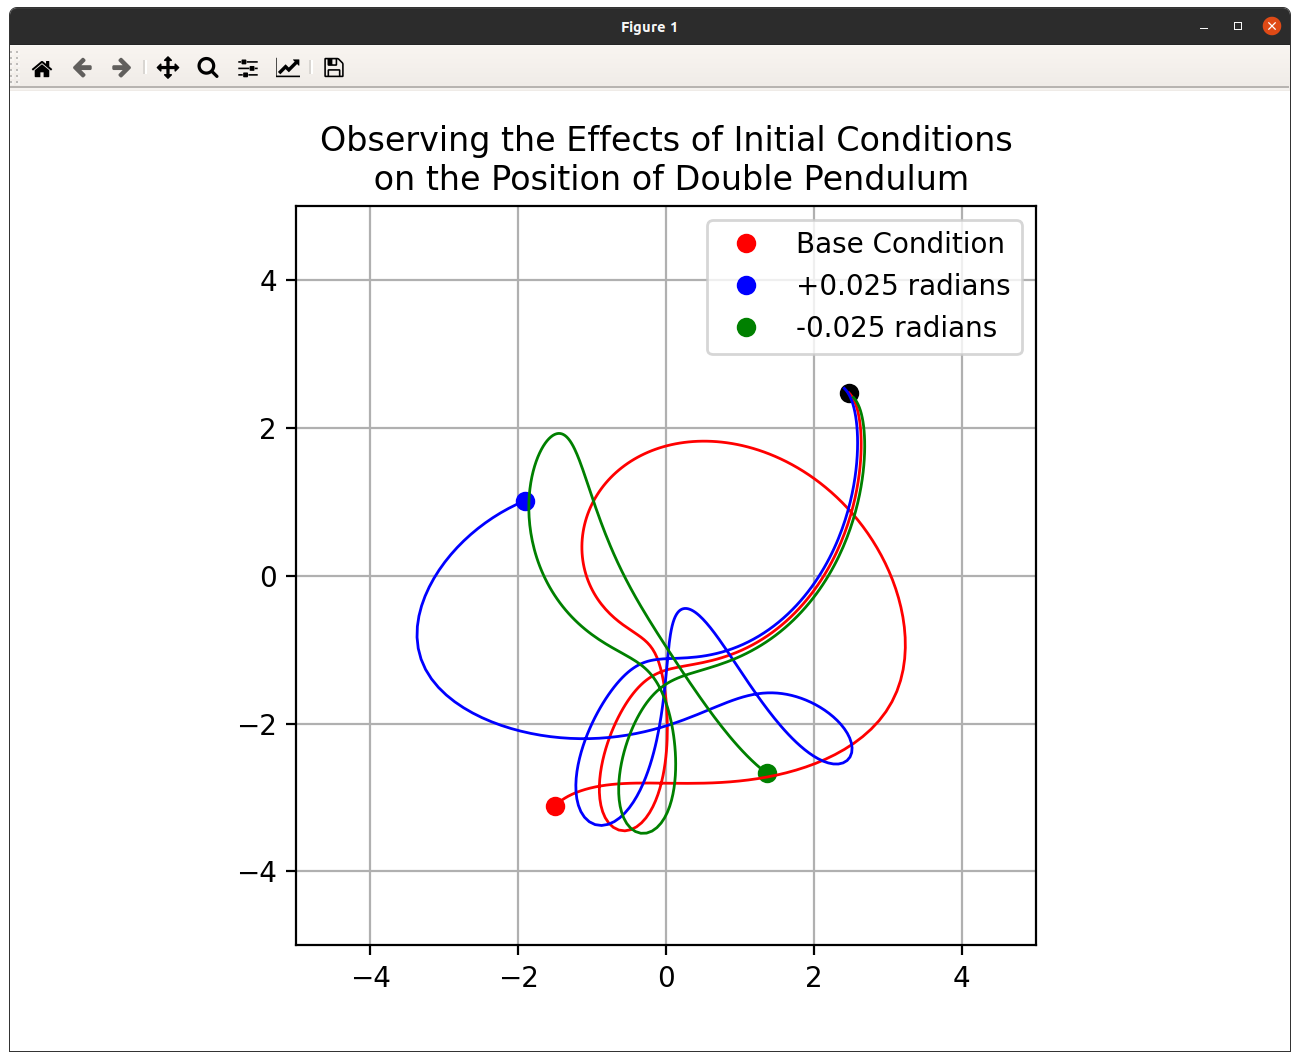
\includegraphics[scale=0.18]{chaos1.png}
    \captionof{figure}{Starting to diverge}
    \label{fig:chaos1}
  \end{minipage}%
  \begin{minipage}{.5\textwidth}
    \centering
    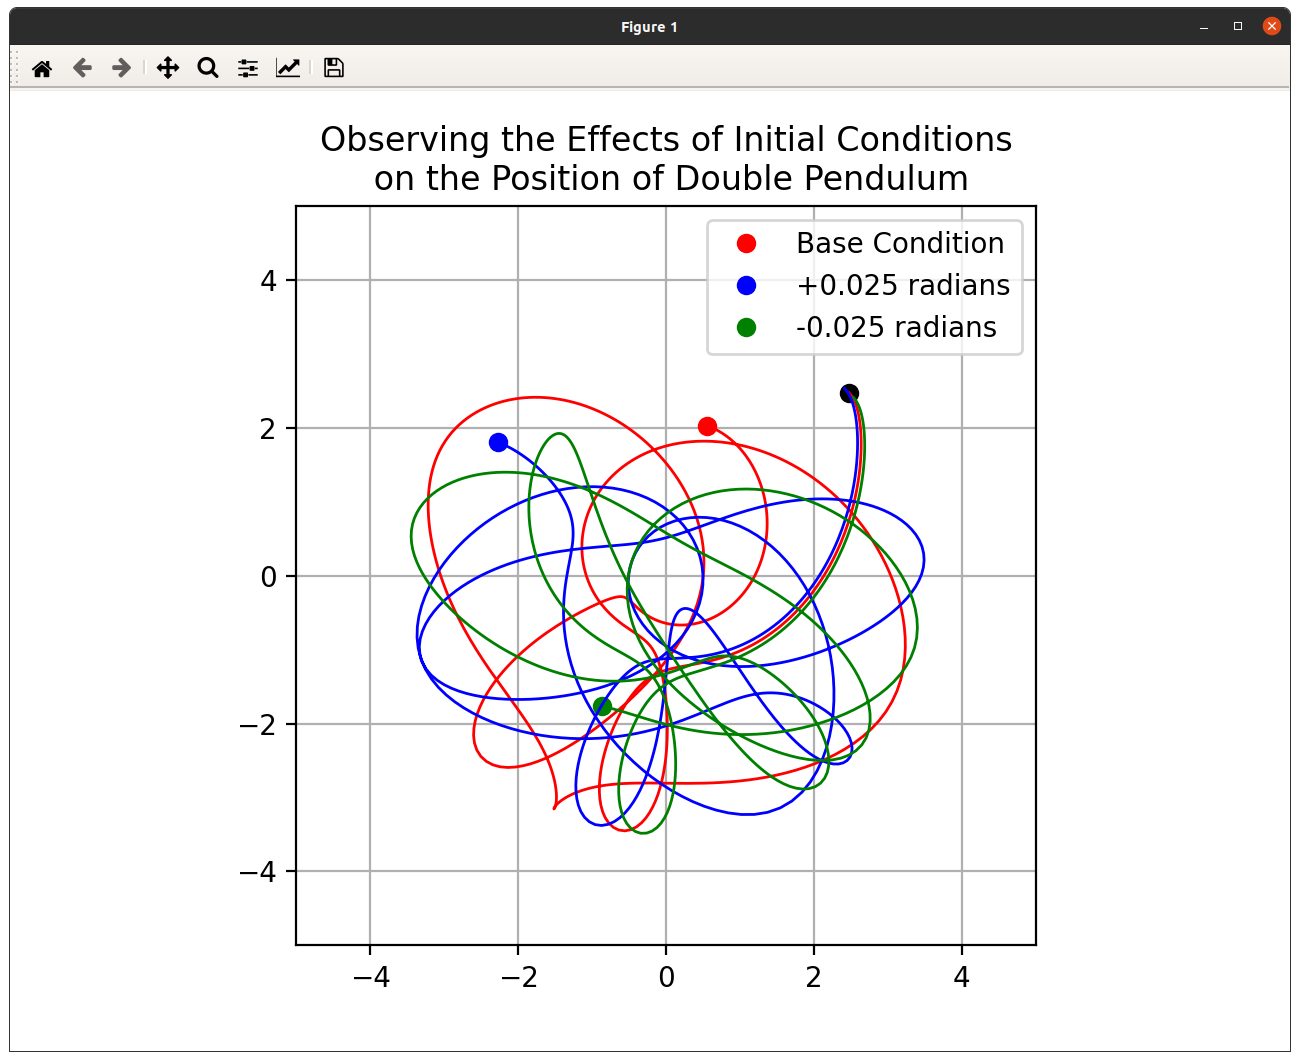
\includegraphics[scale=0.18]{chaos2.png}
    \captionof{figure}{Completely chaotic}
    \label{fig:chaos2}
  \end{minipage}
  \end{figure}

\begin{Example}
  The standard tent map $T(u)=1-|2u-1|$ defined on $[0,1]$ is a common example of a dynamical system satisfying these three properties. 
  \begin{figure}[ht]
    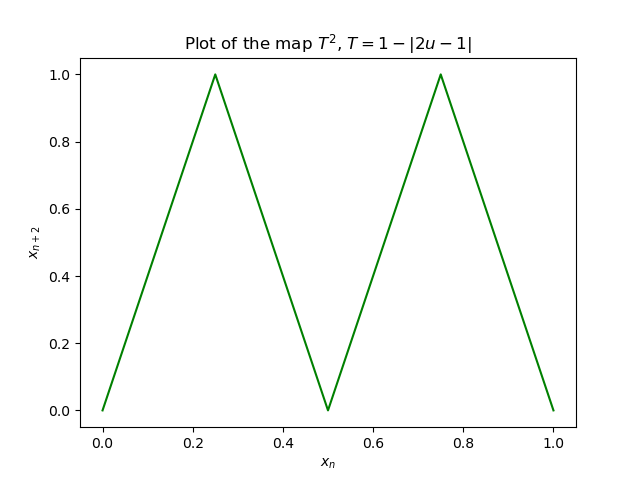
\includegraphics[scale=0.6]{T2.png}
    \centering
    \label{fig:T2tentmap}
  \end{figure}

  Let us now consider why this map exhibit's Devaneys's sense of chaos. The graph of the map $T$ is piecewise linear with two straight lines, one connecting the points $(0,0)$ and $(1/2,1)$ and the other connecting $(1/2,1)$ with $(1,0)$. They form a so-called tent with base centered at $u=1/2$. The graph of the map $T^2$ comprises two symmetric tents with their base centered at $1/4$ and $3/4$.
  % We now reason as why this map exhibits chaos in the sense of Devaney.   
  
  Given any point $u$ and an open neighborhood $W \subset[0,1]$ of $u$, we can find $k\in\mathbb{Z}$ large enough so that $T^k(W) = [0,1]$ because we can accommodate a tent whose base is contained in $W$. \emph{This last phrase doesn't make sense to me.} This implies the existence of two points $w_1$ and $w_2$ in $W$ so that $d(T^kw_1,T^kw_2)= 1$, and by the triangle inequality  at least one of the inequalities $d(T^ku,T^kw_1)> \delta$ or $d(T^ku,T^kw_2)> \delta$ hold when $\delta\in (0,1/2)$. \newline So $T$ has sensitive dependence on initial conditions.  
  
  Next, let $W_1$ and $W_2$ be two nonempty open sets. Given any open set $W_1$, we can find a $k\in\mathbb{N}$ large enough so that $T^k(W_1) = [0,1]$ because we can accommodate a tent with base contained in $W$. So $T^k(W_1) \cap W_2 \not=\emptyset$, and thus $T$ has topological transitivity.
  
  Finally, for every open interval $(a,b)$, the graph of $T^k$ intersects the graph of the identity map on $[0,1]$. This follows from the fact established above that there exists a $k\in\mathbb{N}$ such that $T^k(a,b) = [0,1]$.If the intersection point has coordinates of the form $(p,p)$, the point p is then a fixed point of $T^k$ and therefore also a periodic point of T. It follows that the set of periodic points are dense in T.
  \textbf{Expand further on reason for density.}
\end{Example}





\subsection{Conjugacy}

We now turn our attention to the subject of conjugacy. 

To show topological similarity or sameness between two metric or topological spaces, one needs to establish a homeomorphism between the two spaces. 
However, in the study of dynamical systems defined on two spaces, establishing a homeomorphism does not indicate that the systems are (physically) related in any way. \textbf{"related" - in what sense am I saying it here? Physically?}  For this one rather needs to establish a kind of dynamical equivalence which we illustrate in a simple commutativity diagram below.
% Giving errors
\begin{equation}  \label{eqn_conjugacy}
%    \[ 
    \psset{arrows=->, arrowinset=0.25, linewidth=0.6pt, nodesep=3pt, labelsep=2pt, rowsep=0.7cm, colsep = 1.1cm, shortput =tablr}
 \everypsbox{\scriptstyle}
 \begin{psmatrix}
U & U\\%
V & V.
 %%%
%  \ncline{1,1}{1,2}^{T} 
%  \ncline{1,1}{2,1} <{\phi}
%   \ncline{2,1}{2,2}^{S}
%  \ncline{1,2}{2,2} > {\phi}
 \end{psmatrix}
% \]
\end{equation} 

%Composite functions
To understand the diagram we note that if we travel ``right and then down," the diagram instructs us to use $T$ (top arrow right) first, followed by $\phi$. (right arrow downwards). Consequently the pathway amounts to finding $\phi(T(u))$. If we proceed "down and then right", the diagram instructs us to apply $\phi$ (left arrow downwards) first, and then apply $S$ (bottom arrow right). This then amounts to finding  $S(\phi(u))$. When the relationships in this diagram hold, we say $\phi(T(u))= S(\phi(u))$ and formally denote it as $\phi \circ T=S\circ \phi$.

\begin{Definition}
  Consider the dynamical systems $T:U\to{U}$, $S:V\to{V}$ and suppose the relationship $\phi \circ T=S\circ \phi$ holds. If $\phi$ is a homeomorphism, then S is said to be conjugate to T and $\phi$ is called a conugacy. If we relax the criterion on $\phi$ and merely require $\phi$ to be continuous and surjective, $\phi$ is then a semi-conjugacy between $T$ and $S$; S is said to be semi-conjugate to T. 
\end{Definition}

When $S$ is conjugate to $T$, the dynamics of the two systems are in some way ''dynamically equivalent'' and specifically they are in one-to-one correspondence with one another. However when $S$ is semi-conjugate to $T$ with $\phi$ a many-to-one mapping, the dynamics on $V$ provides a coarse-grained \textbf{cite?} description of the dynamics on $U$ . When $S$ is semi-conjugate to $T$, it is also common to call $S$ a factor of $T$, or conversely that $T$ is an extension of $S$. In essence, an extension (e.g., \cite{de2013elements}) is a larger system capturing all of the important dynamics of its factor.

It is a very hard or nearly an impossible task to establish the existence of a conjugacy or a semi-conjugacy $\phi$ between two systems. \textbf{cite?} However, one can verify that a function $\phi$ satisfies the commutativity diagram \ref{eqn_conjugacy}.  For example $\phi(x)=\sin(\pi x/2)^2$ is a conjugacy between two systems $Tu=1-|2u-1|$ and $Sv=4v(1-v)$  defined on $U=[0,1]$.  

In establishing that two systems are conjugate (semi-conjugate) to one another, we have also shown that one may choose to work with one systems as opposed to the second and still be guaranteed to obtain information on the latter. This is incredibly useful while forecasting the future evolution of dynamical systems. 

\section{The Learning Problem}

\emph{Introduction...}

Consider a relatively simple learning problem: 

Given $(u_0, u_1, \ldots, u_m)$ for $m\in\mathbb{Z}$, a finite segment of an orbit of the map $T$ where $T$ is defined by the update equation $u_{n+1} = Tu_n$, forecast the values $u_{m+1}, u_{m+1}$ where the map $T$ is unknown, given that $u_m$. 

A practical example of this would be - given the sequential coordinates of an object moving in space, predict the future positions of that object. However we are very rarely, if at all, presented with a problem where the entire state information is available to us in the form $u_n$ at some time-step $n\in\mathbb{N}$. Consider then a more involved learning problem:

Suppose we only have the observations $\theta(u_0), \theta(u_1), \ldots, \theta(u_m)$ of the true system states $u$ in an unknown dynamical system $(U,T)$ and we wish to predict the values $\theta(u_{m+1}), \theta(u_{m+2})$. 

Here we consider a continuous-time dynamical system $(U,T)$ with true state $u$ in the input space $U$ and then a measured signal $\theta$ (where $\theta(u_n)=\theta(u(t_n))$ for $n\in\mathbb{N}$. The sequence $\{x_n\}$ represents a scalar time-series and intuitively $\theta$ may be thought to represent a probe inserted into a larger system and itself measuring/extracting only a small part of the greater system state at time $t=n$. Consider for example a thermometer erected to measure the ambient temperature in a local village. This measurement function, the thermometer is capturing a single aspect, the temperature, of a grander dynamical system entailing the present weather of the surrounding area, but even more than that, it is measuring an incredibly small part of the global weather system. 

From here we construct a multidimensional observable using the method of delay-coordinate stacking. 
\textbf{move to later} Given the sequence $\{\theta_1, \theta_2, \ldots\}$, we define the variable \newline $y_n:=[\theta_n, \theta_{n-\tau}, \ldots, \theta_{n-(2d-2)\tau}, \theta_{n-(2d-1)\tau}]^{T}\in\mathbb{R}_{d}\times{1}$ where $\tau$ represents the lag and $d$ the dimension of the attractor. (We shall return to these terms shortly and their discussion may be put on hold for the time being).

However, the true state $u$ of a system is seldom, if ever fully known. In almost all cases we can merely insert probes into a system to obtain partial information by measurements taken. Moreover, the process of taking a measurement itself introduces 2 additional difficulties:
\vspace{-8mm}
\begin{enumerate}[noitemsep, label=\roman*.]
  \item A series of measurements over a specific time-interval is inherently a discretisation
  procedure of the underlying continuous-time dynamical system. (Hence why we restricted our attention to discrete-time systems in the preceding section)
  \item A probe will never be fully accurate and so the act of measurement introduces a certain
measure of numerical noise/inaccuracy.
\end{enumerate}

More formally we may say that in the process of measuring a system, we obtain a 1-dimensional time-series $\{\theta(u(t))\}$, where $\theta:\mathbb{R}^n\to\mathbb{R}$ is a smooth observation or measurement function. This series represents a possibly noise-augmented dataset containing information of certain parts of the original system. 

We may then ask ourselves the question: Is it in any way possible to retain information about the system state $x(t)$ in this temporal data-series $\theta(x(t))$? The answer is easily yes if T is known. However, neither this, nor even the exact function $\theta$ is available. 

\subsection{Taken Embedding Theorem}

We define first the concepts of homeomorphism and embedding:
\begin{Definition}
  A homeomorphism is a function $f:Z\rightarrow Y$ between two topological spaces $Z$ and $Y$ that is continuous, bijective and has a continuous inverse. 
\end{Definition}

\begin{Definition}
  Consider a homeomorphism $f:Z\rightarrow Y$ for $Y\in X$. $Z$ is said to be embedded in $X$ by $f$.
\end{Definition}

Takens Theorem states a result that establishes a relationship between the observed and underlying dynamical systems by showing that the concetantion of a sufficiently large number of previous observations into a vector will, under certain conditions, generate a map between the vectors from the respective systems. \textbf{Check wording} We formultate the theorem from \cite{takens1981detecting}.  

\begin{Theorem} 
	[\bf Takens Embedding Theorem (adopted from \cite{takens1981detecting}] \label{Thm_Takens}
            Let $W$ be a compact manifold of dimension $m$, and $d\ge m$ so that $2d\in\mathbb{Z}$. It is a 
            generic property for the pair $(T, \theta)$,  where $T:W \to W$ is
            a smooth diffeomorphism, and $\theta:W \to \mathbb{R}$ a smooth function, that the map $\Phi_{2d,\theta}:W \to \mathbb{R}^{2d+1}$ defined on $W$ by 
            $\Phi_{2d,\theta}(w) := (\theta(T^{-2d}w)\ldots,\theta(T^{-1}w),\theta(w))$
            is a diffeomorphic embedding; by `smooth' we mean at least $C^2$. Consequently, there exists a map $\Ftheta: \Phi_{2d,\theta}(W) \to \Phi_{2d,\theta}(W)$ defined by 
            \begin{equation}  \label{eqn_takens}
              \Ftheta: (\theta(T^{-2d}w),\ldots,\theta(T^{-1}w),\theta(w)) \mapsto  (\theta(T^{-2d+1}w),\ldots,\theta(T^{-1}w),\theta(Tw))
            \end{equation}
           so that $(W,T)$ is topologically conjugate to 
            $(\Phi_{2d,\theta}(W), \Ftheta)$.   
\end{Theorem} 

(In our scenario, the input space $U$ is considered the attractor.)

Some explanation is beneficial. Takens establishes a delay-coordinate map $\Ftheta$ defined in \ref{eqn_takens} for $T$ the flow (\ref{defn_flow}) defined by the update equation  $Tu_n=u_{n+1}$ and $theta$ our measurement function. When confining a dynamical system to the manifold U (in which the underlying system is contained), Takens showed that if certain smoothness conditions are satisfied on $T$ and $\theta$, then the delay-coordinate map $\Ftheta$ embeds $U$ in the reconstruction space $R^{2d+1}$ \textbf{we haven't used the term reconstruction space yet, so this is falling out of the blue}, for almost every choice of measurement function $\theta$, the observable. By almost every choice here, we mean that we exclude some observations which do not give any information. To see a more precise discussion, see \textbf{xxx} for we do not concern ourselves with a further elaboration on this thesis/report.

Alternatively we may also make the statement: Takens' Embedding Theorem guarantees that almost all dynamical systems can be reconstructed from just one noiseless observation sequence \textbf{this isn't obvious from the theorem's formulation, is it?} i.e. for a great number of possible observation functions $\theta$, $\Ftheta$ preserves the topology of U. \textbf{'preserving the topology' is not something we've touched on before. Perhaps I should add to previous discussion so logic flows seamlessly here}.

\begin{figure}[ht]
  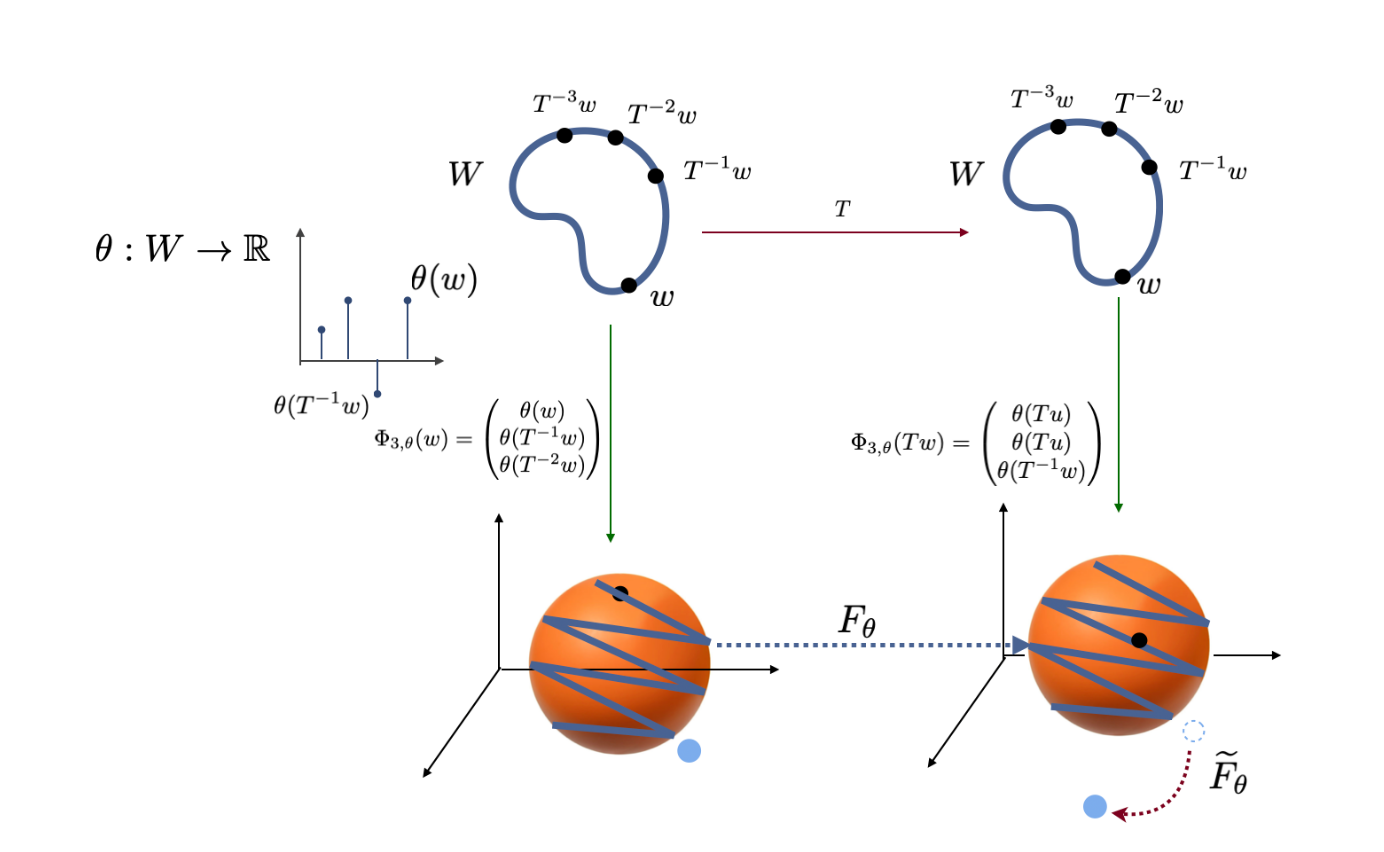
\includegraphics[scale=0.3]{takensmap.png}
  \centering
  \label{fig:takensmap}
\end{figure}

Once again we pause and consider the graph to consolidate our understanding of the conjugacy (\textbf{are we being too simplistic?}). If we are in state $u$ and then evolve towards state $Tu$ before embedding into $\mathbb{R}^{2m-1}$, then this is equivalent to first embedding into $\mathbb{R}^{2m-1}$ and then evolving through the map $\Ftheta$, i.e. $\Phi_{2d,\theta}\circ{F}_{\theta} = T\circ\Phi_{2d,\theta}$. The map $F_theta$ is a homeomorphism as well. 

Thus information about U can be retained in the time series' (or observation's) output. By preserving the topology on the manifold $U$ in the reconstruction space $X$ (\textbf{not discussed before}), we are also guaranteed the preservation of topological invariants of the manifold, of which dimensionality is one such invariant. (We note here that dimensionality will again be considered later in this project/report).

\subsection{Obstacles to Takens}
Despite the fact that the Takens' Embedding Theorem is a powerful result and provides compelling reason to believe that it is possible to accurately ()\emph{right word?}) reconstruct the underlying space, it does present some serious limitations:
\vspace{-5mm}
\begin{enumerate}
\item Even if we can indeed find \Ftheta{}  our \emph{approximation} of \Ftheta{}  is a map from a larger set $\mathbb{R}^{2m+1}$ containing the embedded attractor. There are, however, no theoretical guarantees that \Ftheta{}  will keep this attractor $U$  the same.(\textbf{We haven't properly said that U is an attractor, or have we.})
\item Takens only holds for noiseless observations. Suppose the case where \Ftheta{} was learnt, but due to measurement error or other noise we obtained the set $V$ and not the original attractor. Due to the chaotic nature of the underlying system (i.e. the fact that it has SIDC), this new system $V$ will then move in a different direction. This problem will later be eliminated by some properties of a new function $g$, namely the Unique Solution Property. 
\item It is an unfortunate case that the functional complexity (i.e., the relative number of oscillatory graphs \cite{manjunath2021universal}) as well as stability of the embedding \Ftheta{} (\textbf{cite?})depends on the choice of observable $\theta$. This means that we may even learn a map that complicates our learning task and in so doing adds obstacles to the road to learning a conjugate map with predictive power. (\textbf{Am I talking nonsense here?})
\end{enumerate}

Another limitation owes itself to the requirement that T be a surjective map. This is not always the case in practical examples and we may consider the case of a damped double pendulum. 

\textbf{Continue writing here}


\begin{figure}[ht]
  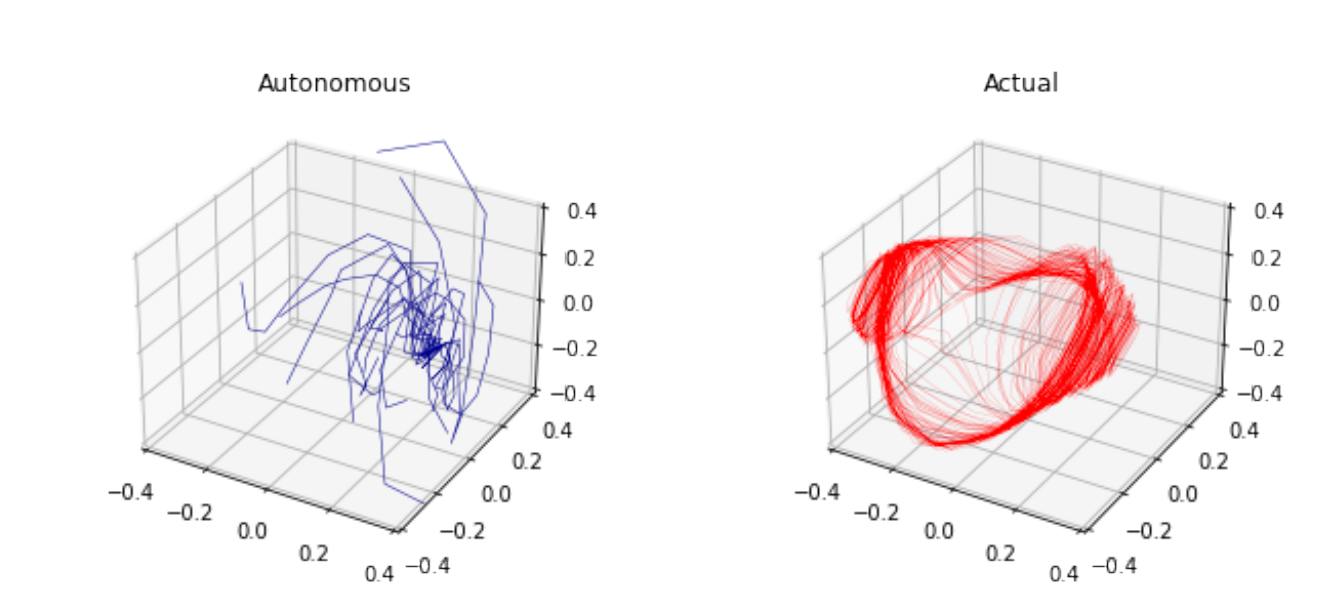
\includegraphics[scale=0.3]{learningfailure.png}
  \centering
  \label{fig:supp_learning_failure}
  \caption{Illustration of a system having failed to learn the map}
\end{figure}


\textbf{Explanation continued here}

\begin{figure}[h]
  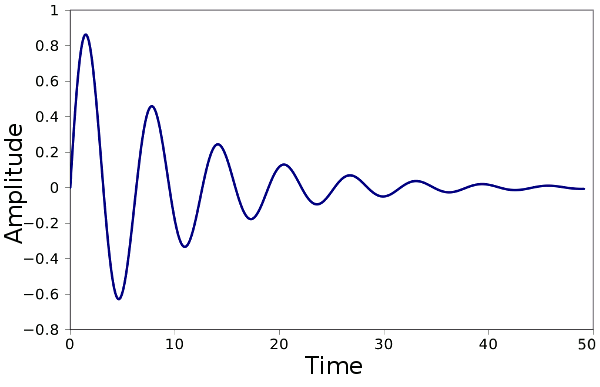
\includegraphics[scale=0.4]{temporary_damp_fig.png}
  \centering
  \label{fig:damped_pendulum}
\caption{A damped pendulum}
\end{figure}

\textbf{Continue explaining here}


\section{Obtaining X through Driven Dynamical Systems}

In this chapter, we recall results on mapping temporal data acquired from a discrete-dynamical system onto a different space through a driven dynamical system. We recall the conditions the driven system should have not to add distortion to its state space representation, so that the single-delay dynamics (SDD) gets conjugate or semi-conjugate to the system. The SDD can be then use to forecast and reconstruct the underlying attractor

\subsection{Nonautonomous and Driven Dynamical Systems}

A nonautonomous dynamical system is simply a dynamical system where the input $u$ from the input space $U$, a  topological space is time-dependent. \textbf{This means it can no longer be generated by a flow?}

We now recall the figure first defined in \ref{eqn_conjugacy} below and the greater goal to construct a system - such as $(V,S)$  - conjugate to $(U,T)$, 

%#####################################
\begin{center}
\psset{arrows=->, arrowinset=0.25, linewidth=0.6pt, nodesep=3pt, labelsep=2pt, rowsep=0.7cm, colsep = 1.1cm, shortput =tablr}
\everypsbox{\scriptstyle}
\begin{psmatrix}
U & U\\%
V & V.
%%%
%  \ncline{1,1}{1,2}^{T} 
%  \ncline{1,1}{2,1} <{\phi}
%   \ncline{2,1}{2,2}^{S}
%  \ncline{1,2}{2,2} > {\phi}
\end{psmatrix}
%#####################################
\end{center}

To do this, we need to consider a driven dynamical system taking input from both an input space $U$, and an underlying state space $X$. This is done to account for influence of both the input and the actual state of the system at a specific timestep.

\begin{Definition}
A driven dynamical system comprises two topological spaces $U$, $X$ and a continuous function  $g:U\times{X}\to{X}$ where $g(u_n, x_n)=x_{n+1}$. The dynamics on X are generated by the update equation $x_{n+1}=g(u_n, x_n)$ where $n\in\mathbb{Z}$, $u_n$ from the metric input space $U$ and state $x_n$ belonging to the state space $X$, a compact metric space. If the input space $U$ is compact, we refer to the system as compactly driven. 
Abbreviated, we shall refer only to the "driven system $g$", with all other entities being understood implicitly.
\end{Definition}

In particular, a nonautonomous dynamical system may be generated from $U$; any input $\overline{u}$, a bi-infinite sequence from $U$ gives rise the sequence of self-maps $\{g(u_n, \ldotp)\}_{n\in\mathbb{Z}}$ contained in $X$. \textbf{explain better why}
Physically, one may think of this bi-infinite as referring to a system that has been running for an incredibly long period at the time of the first measurement/observation taken from the system.

\begin{Definition}
  A sequence $\{x_n\}_{n\in\mathbb{Z}}\subset{U}$ is called an entire solution(or simply a solution) to the driven system  $g$ with input $\overline{u}$ when it satisfies 
  $$g(u_{n-1}, x_{n-1})=x_n$$ for all $n$ in $\mathbb{Z}$
\end{Definition}

It is important to emphasise that a sequence satisfying the update equation above can only be a solution if $x_n\in{U}$ for all $n\in\mathbb{Z}$. Consider the example below.

\begin{Example}
  Consider the driven system $g(u_n,x_n)=x^n$ for $X=[0,1]$. This system has an uncountable number of solutions, because for every $x\in{X}$, there exists a solution passing through the point $x$ and $lim_{n\to\infty}x_n=0$, $lim_{n\to{-}\infty}x_n=1$.
\end{Example}

\begin{Definition}
Let $X_n{\overline{u}}:= \cap_{m<n}{\phi_{\overline{u}}(n,m,X)}$ be the set of all reachable states at time $n$ for input $\overline{u}$.
  A function $g:U\times{X}\to{X}$ is a topological contraction if for all $n\in\mathbb{Z}$ and all $\overline{u}\subset{U}$, $X_n(\overline{u})$ is a singleton subset of X.  
\end{Definition}

Note that $x\in{X_n{\overline{u}}}$ if and only g has a solution $\{x_k\}$ s.t. $x_n=x$ and the input is $\overline{u}$. \textbf{cite paper}. This will lead to a result established later, but which is worth taking note of now: $g$ being a topological contraction is equivalent to the existence of a unique entire solution for every $n\in\mathbb{Z}$. \textbf{Adding worth or not?} \label{here_UAP_firstestablished}

\begin{Example}\label{ex_halfux}
  If $X=[0,1]$, $U=[0,1]$, then the only possible solution $\{x_n\}$ to the driven system $g(u,x)=\frac{ux}{2}$ is the zero solution $x_n\equiv0$.

  To see this, we show that for every input $\{u_n\}$, $g(u_k,\dot)$ is a contraction map on $X$ for every $k\in\mathbb{Z}$. \textbf{Show}
  Consequently, we easily conclude that $\{x_n\}$ where $x_n=0$ for all $n\in\mathbb{Z}$ is the only solution. \textbf{Show}
\end{Example}

One may ask if a driven system always has a solution, and if so, whether it has certain properties such as uniqueness. Should the system be compact, existence follows immediately as can be seen in the following result.

%%%%%%%%%%%%%%%%%%%%%ISSUE HERE - fix before sending
\begin{Theorem}
  If $X$ is compact then for each input $\overline{u}$, there exists at least one solution to the driven system $g(\ldotp, x)$
\end{Theorem}
\begin{proof}
  Consider ${u_n}_{n\in\mathbb{Z}}\subset{U}$ and $g:U\times{X}\to{X}$  generating a sequence ${x_n}_{n\in\mathbb{Z}}$ in the compact space. (If U is a metric space then $x_n$ has a convergent subseqeunce)
\end{proof}

\begin{Example}
  The driven system $g(u,x)=x$ has only the constant solution $x$ and so for $U=[-1,1]$, the system has no solution if $|X|>1$
\end{Example}

The examples above present systems with trivial sets of solutions. To refine the scenario, we define systems with unique solutions. 

\begin{Definition}
  A driven system $g$ is said to have the Unique Solution Property if for each input $\overline{u}$ there exists exactly one solution. Alternatively we may formulate the USP as follows: $g$ has the Unique Solution Property if there exists a well-defined map $\Psi:{U}\to{X}$ where $\Psi({\overline{u}})$ denotes the unique solution 
\end{Definition}

\emph{(More discussion on USP … - not yet filled in ...)}

We next identify a subspace $X_U$ of $X$ that contains all possible solutions. To realize such a subspace of a driven system $g$, we define 
the \textit{reachable set} of the driven system $g$ to be the union of all the elements of all the solutions, i.e., 
$$X_U :=\Big \{x \in X:  x = x_k \mbox{ where  $\{x_n\}$  is a solution for some  $\bar{u}$} \Big \}.$$

We denote $\cev{u}^{n}:=(\ldots,u_{n-2} ,u_{n-1})$ and $\overleftarrow{U}$ denote all the left-infinite sequences in $U$. 
Symbolically we let $\cev{u}^{n}v:=(\ldots,u_{n-2} ,u_{n-1}, v)$ denote the input up to time $n$ with $v \in U$ being the input value at time $n$. This introduction of a new input at time $n$ can be described by a mapping $\sigma_v:   
\cev{u}^{n} \mapsto \cev{u}^{n}v$.   \textbf{Is this in the right place?}


The question now becomes whether we may establish a conjugacy as presented below for g driven

\begin{equation}  \label{Scomm_h}
  %    \[ 
      \psset{arrows=->, arrowinset=0.25, linewidth=0.6pt, nodesep=3pt, labelsep=2pt, rowsep=0.7cm, colsep = 1.1cm, shortput =tablr}
   \everypsbox{\scriptstyle}
   \begin{psmatrix}
   \overleftarrow{U} & \overleftarrow{U}\\%
   X_U & X_U.
   %%%
  %  \ncline{1,1}{1,2}^{\sigma_v} \ncline{1,1}{2,1} <{h}
  %  \ncline{1,2}{2,2} > {h}
  %  \ncline{2,1}{2,2}^{g(v,\cdot)}
   \end{psmatrix}
  % \]
  \end{equation} 	


  \begin{Definition} \rm \label{Def_UC}
    Given a driven system $g$, we  call a continuous and surjective map $h : \overleftarrow{U} \to X_U$ a universal semi-conjugacy if  diagram \ref{Scomm_h} commutes for all $v \in U$.
  \end{Definition}

If the universal semi-conjugacy $h$ exists (i.e. the diagram  \ref{Scomm_h} commutes) then the solution $\Psi$ will be at least a coarse-grained representation of the input $u$; we may now consider the question of the existence of such a function $h$ for the driven system defined above. 

If $g$ has the USP and $\Psi(u)=\{x_n\}$ then $h$, defined by  $h(\overleftarrow{u}_n)=x_n=g(u_n,x_{n-1})$, will satisfy the semi-conjugacy in the graph above \ref{Scomm_h}.

In general the mapping h is not guaranteed to exist. We thus state the following result.

\begin{Theorem}
  For a compactly driven system, a causal mapping $H$ exists if and only if $g$ has the USP. 
\end{Theorem}
\begin{proof}
  \emph{See proof from p.15 of \cite{manjunath2021universal}}
\end{proof}

Note that even when $h$ does exist, we are not guaranteed its injectivity. Considering again example 3* \ref{ex_halfux}, we conclude that even if $h$ were to exist, it could not be injective as $X_U=\{0\}$. 

An embedding of the space $\overleftarrow{U}$   would allow one to establish topological conjugacy, which in turn provides stronger results than merely obtaining a coarse-grained representation via a causal mapping. 

Re-sketching the graph \ref{Scomm_h} above by fixing $v$ in $g$ and replacing $X_U$ by its left-infinite sequence space $\overleftarrow{U}$, we obtain the graph below. In this case, the function $H:\overleftarrow{U}\to\overleftarrow{X}_U$, a map that is both continuous and surjective, is called a \emph{causal mapping}. 

\begin{equation}  \label{SCausal_H}
    %    \[ 
        \psset{arrows=->, arrowinset=0.25, linewidth=0.6pt, nodesep=3pt, labelsep=2pt, rowsep=0.7cm, colsep = 1.1cm, shortput =tablr}
     \everypsbox{\scriptstyle}
     \begin{psmatrix}
     \overleftarrow{U} & \overleftarrow{U}\\%
     \overleftarrow{X}_U & \overleftarrow{X}_U.
     %%%
    %  \ncline{1,1}{1,2}^{\sigma_v} \ncline{1,1}{2,1} <{h}
    %  \ncline{1,2}{2,2} > {h}
    %  \ncline{2,1}{2,2}^{\tilde{g}_v}
     \end{psmatrix}
    % \]
    \end{equation} 	

  Note that $\tilde{g}_v$ maps $(\ldots, u_{-2}, u_{-1})$ to $(\ldots, u_{-2}, u_{-1}, g(v, u_{-1}))$.
  The driven system $g$ can induce an embedding of $\overleftarrow{U}$ in $\overleftarrow{X}$ as follows: 
  If $H$ is also injective (and hence bijective), it becomes the embedding of $\overleftarrow{U}$ in $\overleftarrow{X}$ induced by the driven system $g$ and we refer to $H$ as a \emph{causal embedding}. We formalise this in the following definition.

\begin{Definition}
  A driven system $g$ is said to causally embed the dynamical system $(U,T)$ if 
  \vspace{-8mm}
\begin{enumerate}[noitemsep, label=\roman*.]
  \item The diagram below commutes (i.e. $g$ is a universal semi-conjugacy),
  \item $H_2(\overline{u}):=(h(r\overline{u}, h(\overline{u})))$ embeds the inverse-limit space $(\hat{U}, \hat{T})$ of $(U,T)$ in $X\times{X}$.
\end{enumerate}
\end{Definition}


\begin{Theorem}
 If $g(\ldotp,x)$ is invertible and has the USP then $H$ is a causal embedding. 
\end{Theorem}

When g has the USP, the diagram below illustrates the operation of the the mappings h and H the mapping $h:\overleftarrow{U}\to{X_U}$ is an observable as discussed (above).  

\begin{figure}[ht]
  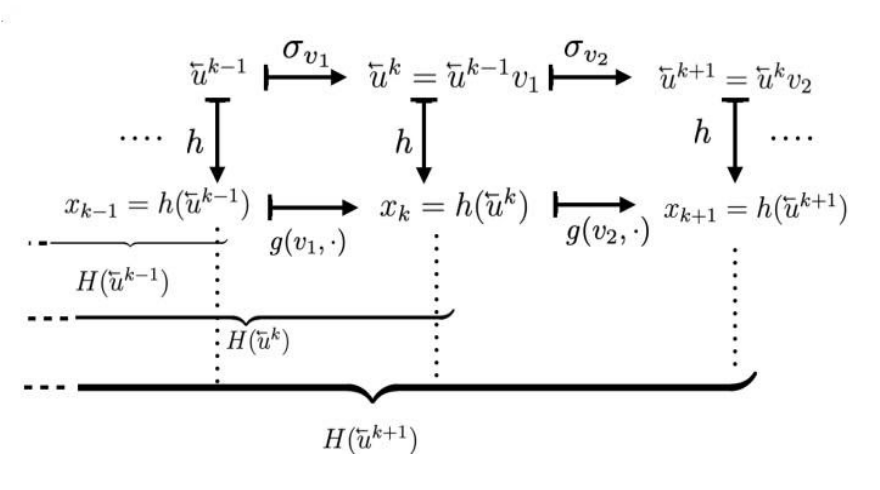
\includegraphics[scale=0.3]{actionofh_H.png}
  \centering
  \label{fig:actionh_H}
\end{figure}

\begin{Theorem}
  The following statements are equivalent:
  \vspace{-8mm}
  \begin{enumerate}[noitemsep, label=\roman*.]
    \item $g$ has the USP 
    \item $g$ is topological contraction 
    \item $g$ has the Unique Attraction Property (UAP). 
  \end{enumerate}
\end{Theorem}
\begin{proof}
  (we’ll show this)  [11] eqn.6 
\end{proof}

We have not as of yet treated the UAP, and establish the necessary result here (without proof - left to literature or later) so as not to break up the completeness of theorem 

It is important to note here that one must be careful to avoid a choice of g which adds additional complexity to the obtained solution.  
When the causal embedding exists for the driven system $g$, one may map an arbitrary input $u$ onto the solution space $X$ without additional distortion or information-loss.  
Establishing an embedding removes this problem by guaranteeing that, since the systems are conjugate (semi-conjugate), $g$ does not add any (only “some”) complexity to the system.  
It is, however, a balancing act as one also does not want to choose a function g that quenches the temporal structure in $u$ by contracting to such a degree that one loses the ability to recover information from the original system completely. To obtain this we want the reachable set of a driven system to be large enough to relate to the input.  
 
In the example above \ref{ex_halfux}, we cannot relate the input's temporal variation and the reachable set because $X_U$ consists of a single element.  

The reachable set $Y_T$ of a driven system must therefore be such that we can embed the inverse-limit space of $U_T$ can be embedded in some finite self-product of the reachable set of $T$. To this end, consider the notion of State-Input (SI) Invertibility.  

\begin{Definition}
  A map $g$ is said to be SI-Invertible if $g$ is invertible for all $x\in{X}$. Alternatively, if, given $x_n$ and $x_{n-1}$, $u_n$ can be uniquely determined from $x_n=g(u_n,x_{n-1})$, then $g$ is said to be SI-invertible.
\end{Definition}
 
We make special note of a specific driven system. The function $$g(u,x)=(1-a)x+atanh(Au+\alpha{a}Bx)$$  is both SI-invertible and possesses the USP. This function $g$ is used in our implementation and is more completely discussed in Section 5 \ref{sect5}
The proof of these two facts is rather involved and the proof, instead of being replicated here, may be found in (cite relevant article) 


\textbf{Expand: UAP + Embedding -> perturbation isn’t an issue + we can drop left-infinite sequence.  }

Despite the ease that one may work with left-infinite sequences in the realm of theory, it is impossible to obtain such a sequence in any real-life application.  One does not in practice, however, need the entire left-infinite history of the input due to the Uniform Attraction Property (UAP). The next definition is stated in an informal manner as the more rigourous definition makes use of processes, a concept which would take some amount of paper to establish and explain - something which would detract from the overarching thrust of this paper/project/thesis. \textbf{is it VERY obsious to the reader at this point what the general 'thrust' of the paper IS?} \textbf{Cite articles}

\begin{Definition}
  A driven system $g$ has the Uniform Attraction Property (UAP) if, regardless of starting position, all trajectories converge to a single trajectory as time flows forward. 
  This trajectory is also the unique solution sequence $x$ to the input sequence $u$ as mentioned above \ref{here_UAP_firstestablished}.
\end{Definition}

Incredibly, one may then initialise a driven system with a completely arbitrary initial value $y_m\in{X}$ where $m\in\mathbb{Z}$ and the UAP then guarantees that the sequence $\{y_{m+1}, y_{m+2},\ldots\}$ satisfying $y_n=g(u_n, y_{n-1})$  with $k\geq{m}$  will uniformly approach the elements $\{x_n\}$ of the actual solution. (see [41, Theorem 1] or [11, Eqn. (18)]) 
 
One may now appreciate an even more astounding result. $g$ having the USP is equivalent to the UAP and so one need not establish any additional results to ensure that the sequence uniformly approach the unique solution $\Psi$. This vastly simplifies the work needed to be done in setting up a problem to guarantee that the underlying system will be accurately 'represented' by the conjugate system. \textbf{Check this statement again to make sure it's not nonsensical.} 

\begin{figure}[h]
  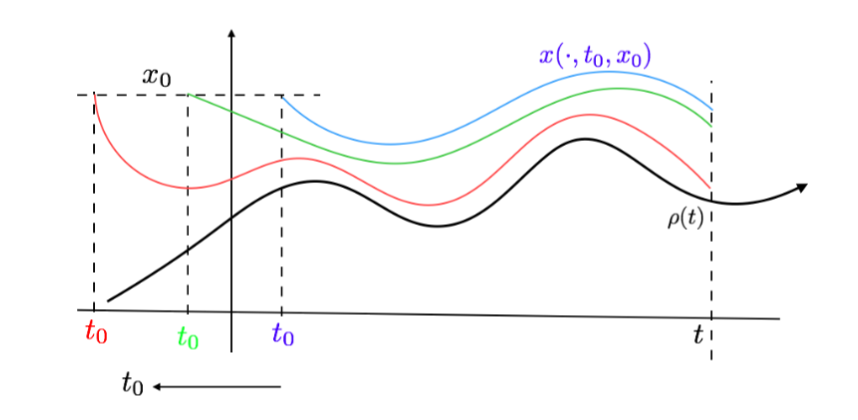
\includegraphics[scale=0.4]{memloss_conttime.png}
  \centering
  \label{fig:memoryLosscont_time}
%\caption{Approaching the true solution if g has the UAP}
\end{figure}

This also solves the problem of perturbations or noise introduced by the observable or measurement function. \textbf{(rephrase)}

Next we define the relation $Y_T$ induced by $(U,T)$ on $X_U\times{X_U}$ for a driven system $g$ possessing SI-invertibility.  To describe the  single-delay lag dynamics formally, we consider a dynamical system $T: U \to U$ and we define a relation on the reachable set $X_U$, i.e., a subset defined on $X_U \times X_U$ by 
$$Y_T:=\{(x_{n-1},x_n): \{x_k\}_{k\in \mathbb{Z}} \mbox{ is a solution for some orbit of } T \mbox{ and } n \in \mathbb{Z}\}.$$ 

The following theorem establishes the existence of a well-defined map GT describing the single-delay dynamics of the system above. 

\begin{Theorem}
If we let $G_T:Y_T\to{Y_T}$ be a map defined by the relation $(x_{n-1},x_n)\mapsto(x_n,x_{n-1})$, then $G_T$ is well-defined (and this results holds even in the absence of $g$ possessing over the USP)  
\end{Theorem}


We're not getting quite close to where we want to be and our results carry more and more weight. Recall that $g$ is only being given inputs from the orbits of $T$.  

\begin{Theorem}
  Graph 1 is exactly the inverse-limit system $(\hat{U}, \hat{T})$.    
\end{Theorem}



%%%%%%%%%%%%%%%%%%%%%%%%%%%%%%%%%%%%%%%%%%%%%%%%%%%%%%%%%%%%%%%%

\section{Implementation} \label{sect5}
 
 



\vspace{-1cm}
\bibliographystyle{pnas-new}
\bibliography{pnas}




\end{document}